\documentclass[tikz,border=5pt]{standalone}
\usepackage{fourier}
\usetikzlibrary{bending,patterns.meta}
\begin{document}
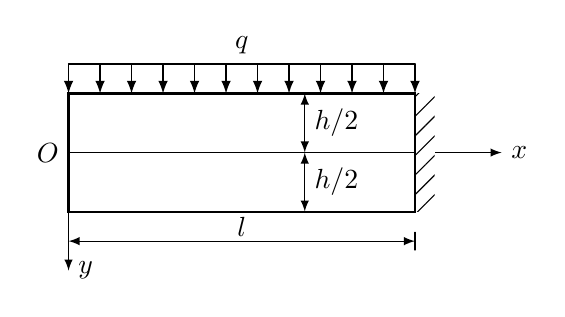
\begin{tikzpicture}[>=latex,line cap=round,yscale=.75]
    \draw[->] (0,0) node[left] {$O$} -- (5.5,0) node[right] {$x$};
    \draw[->] (0,0) -- (0,-2) node[right] {$y$};
    \fill[pattern={Lines[angle=45,distance={5pt}]},preaction={fill=white}] (4.4,-1) rectangle ++(.25,2);
    \draw[thick] (4.4,1) rectangle (0,-1);
    \draw (0,1.5) -- node[above] {$q$} ++(4.4,0) (4.4,-1.35) -- ++(0,-.3);
    \draw[<->] (0,-1.5) -- node[above=-2pt] {$l$} ++(4.4,0);
    \draw[<->] (3,0) -- node[right] {$h/2$} ++(0,1);
    \draw[<->] (3,0) -- node[right] {$h/2$} ++(0,-1);
    \foreach \i in {0,.4,...,4.4}{
        \draw[->,semithick] (\i,1.5)-- ++(0,-.5);    
    }
\end{tikzpicture}
\end{document}